%\documentclass[12pt,handout]{beamer}
%\documentclass{beamer}
\usepackage[ngerman]{babel}
\usepackage[utf8]{inputenc}
\usepackage{amsmath}
\usepackage{amssymb}
\usepackage{listings} 
\usepackage{stmaryrd}
\lstset{language=Python, tabsize=4, showstringspaces=false,basicstyle=\footnotesize,mathescape=true}
\lstset{literate=%
  {Ö}{{\"O}}1
  {Ä}{{\"A}}1
  {Ü}{{\"U}}1
  {ß}{{\ss}}1
  {ü}{{\"u}}1
  {ä}{{\"a}}1
  {ö}{{\"o}}1
}  
\usepackage{mathtools}
\usepackage{ulem}
\usepackage{tikz}

\usetheme{Boadilla}
\mode<presentation>{
\useoutertheme[subsection=false]{miniframes}
\useinnertheme{rectangles}
%\usecolortheme{crane}
}
\parskip 10pt



\begin{document}
\title{Informatik}   
\author{Spielbaum} 
\date{}
\frame{\titlepage} 
\small
%---
\begin{frame}[fragile]

In einem \textbf{Mehrwegebaum} kann jeder Knoten eine variable Anzahl von Söhnen besitzen. 


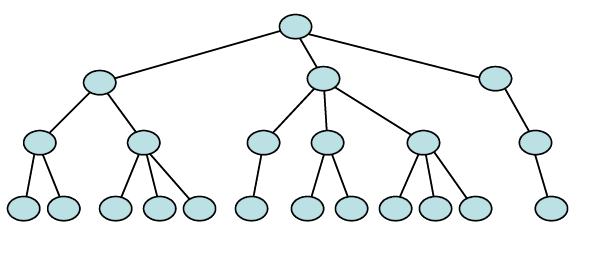
\includegraphics[width=10cm]{bild1a.png} 

\end{frame}


\begin{frame}[fragile]
Ein \textbf{Spielbaum} ist ein Mehrwegebaum mit zwei Typen von Knoten: Minimum-Knoten und
Maximum-Knoten.  \pause

Die Knoten repräsentieren Spielstellungen. 

Die Kanten zwischen den Knoten repräsentieren Spielzüge. \pause

Der Spielbaum eignet sich für Zwei-Personen Nullsummenspiele wie Schach, Dame, TicTacToe, wo 2 Personen
 abwechselnd ziehen und der Gewinn des einen Spielers dem Verlust des anderen Spielers entspricht. \pause
 
Der Wert eines Minimum-Knotens ist das Minimum der Werte seiner Söhne. 
Der Wert eines Maximum-Knotens ist das Maximum der Werte seiner Söhne.   \pause

Der Wert eines Blattes wird bestimmt durch eine statische Stellungsbewertung.
\end{frame}

\begin{frame}[fragile]
Beispiel für einen Spielbaum

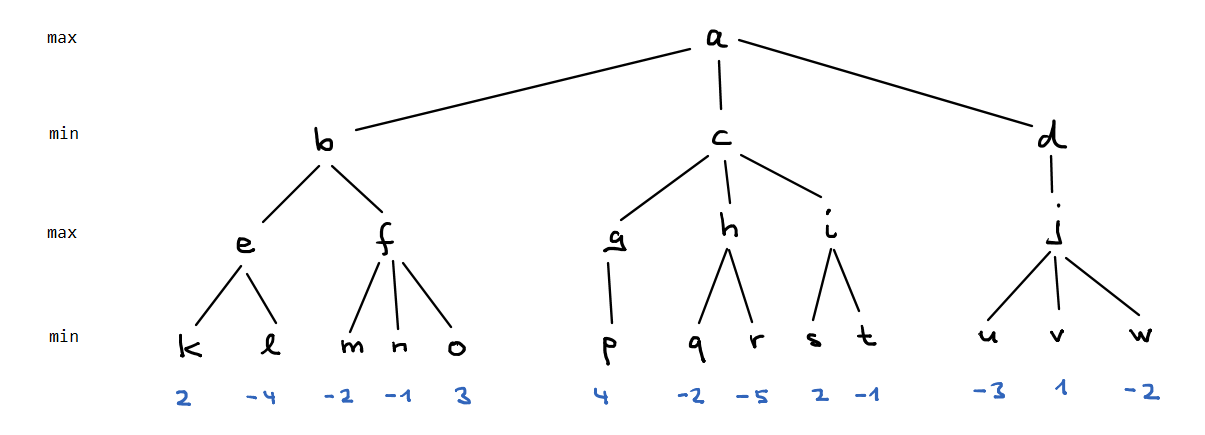
\includegraphics[width=12cm]{bild10.png} 

\end{frame}

\begin{frame}[fragile]


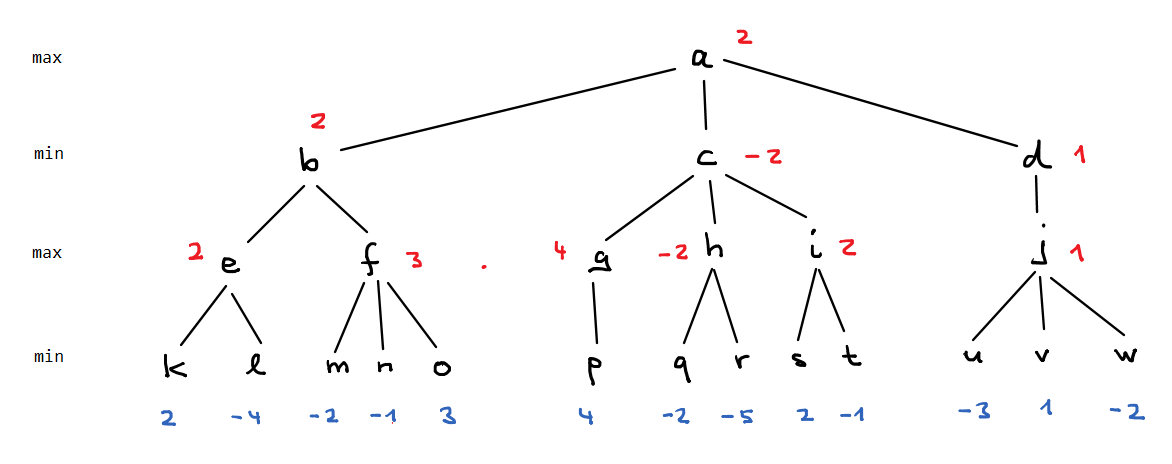
\includegraphics[width=12cm]{bild11.png} 

Reihenfolge, in der die Knoten ihre 
Bewertung erhalten:

e:2 f:3 b:2 g:4 h:-2 i:2 c:-2 j:1 d:1 a:2 \\
bester zug: b

\end{frame}

\begin{frame}[fragile]
Der MinMax-Algorithmus
\begin{lstlisting}[basicstyle=\tiny]
def maximize(state):
    '''
    state: Spielstellung
    returns: (st, k), die Folgestellung st, die die höchste Bewertung k hat
    '''
    Falls state ein Blatt ist, wird keine Folgestellung sondern nur die 
        Stellungsbewertung zurückgegeben.
    
    Von allen Kindern von state wird das mit der höchsten
    Bewertung des Minimizers zurückgegeben.
\end{lstlisting} 
\begin{lstlisting}[basicstyle=\tiny]
def minimize(state):
    '''
    state: Spielstellung
    returns: (st, k), die Folgestellung st, die die niedrigste Bewertung k hat
    '''
    Falls state ein Blatt ist, wird keine Folgestellung sondern nur die 
        Stellungsbewertung zurückgegeben.
    
    Von allen Kindern von state wird das mit der niedrigsten
    Bewertung des Maximizers zurückgegeben.
    
st =  ...                      # Ausgangsstellung
besterZug, k = maximize(st)    # der beste Zug nach st für den Maximizer
\end{lstlisting} 
\end{frame}

\begin{frame}[fragile]
Für Implementierung des MinMax-Algorithmus setzen wir folgende Funktionen voraus:
\begin{lstlisting}[basicstyle=\tiny]
def nextstates(state):
    '''
    state: Spielstellung
    returns: Liste mit möglichen Folgestellungen
    '''

def terminal_test(state):
    '''
    state: Spielstellung
    returns: True, wenn Stellung ein Blatt ist
    '''

def evaluation(state):
    '''
    state: Spielstellung
    returns: Zahl, die den Wert der Stellung wiedergibt
    '''
\end{lstlisting} 
Mit diesen Funktionen können wir die Funktionen maximize und minimize implementieren unabhängig von 
der konkreten Instanz des MinMax-Problems.
\end{frame}

\begin{frame}[fragile]
\begin{lstlisting}[basicstyle=\tiny]
inf = float('inf')
def maximize(state):
    if terminal_test(state):
        return None,evaluation(state)
    v, bestChild = -inf, None
    for child in nextstates(state):
        _,utility = minimize(child)
        if utility > v:
            bestChild,v = child,utility
    return bestChild,v

def minimize(state):
    if terminal_test(state):
        return None,evaluation(state)
    v, bestChild = inf, None
    for child in nextstates(state):
        _,utility = maximize(child)
        if utility < v:
            bestChild,v = child,utility
    return bestChild,v

# bester folgezug für maximizer nach state
bestnext, _ = maximize(state)

# bester folgezug für minimizer nach state
bestnext, _ = minimize(state)
\end{lstlisting} 
\end{frame}

\begin{frame}[fragile]
 
Beispiel-Spielbäume geben wir mit zwei dictionaries an:
\begin{lstlisting}[basicstyle=\tiny]
nxt = {'a':list('bc'),'b':list('de'),'c':list('fg')}   # wurzel 'a'
blatt = {'d':10,'e':8,'f':4,'g':50}
 
def nextstates(state):
    return nxt[state]
        
def terminal_test(state):
    return state in blatt

def evaluation(state):
    return blatt[state]
\end{lstlisting} 

\pause
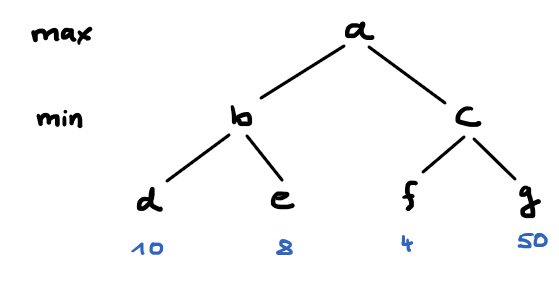
\includegraphics[width=5cm]{minmax_folie01.png} 

Reihenfolge der besuchten Knoten (ohne Blätter):  b:8 c:4 a:8 \\
Bester Zug: b
\end{frame}



\begin{frame}[fragile]
Für ein konkretes Spiel müssen wir uns entscheiden, wie wir eine Spielstellung repräsentieren. Anschließend müssen wir die drei Funktionen \texttt{nextstates, terminal\_test} und \texttt{evaluation} implementieren.

Beispiel: Tic-Tac-Toe

Es gibt mehrere Möglichkeiten, eine Spielstellung zu repräsentieren.
\begin{lstlisting} 
x . . 
. o . 
. . . 
\end{lstlisting}  \pause
- Matrix mit Zeichen: \texttt{[['x','.','.'],['.','o','.'],['.','.','.']]} \\
- Matrix mit Zahlen:   \texttt{[[1,0,0],[0,-1,0],[0,0,0]]} \\
- Liste mit Tupeln: \texttt{[(0,0),(1,1)]} \\
- Liste mit Zahlen: \texttt{[0,4]} \\
usw.

\end{frame}

\begin{frame}[fragile]
Beispiel: Liste mit Zahlen, d.h. die Felder des Spielfeldes werden von 0 bis 8 durchnummeriert.
\begin{lstlisting} [basicstyle=\tiny]
def nextstates(state): $\pause$
    temp = []
    for i in range(9):
        if i not in state:
            temp.append(state+[i])
    return temp    $\pause$

def evaluation(state): 
    '''
    state: Stellung
    returns: Zahl, die den Wert der Stellung wiedergibt
       +1 Maximizer gewinnt, -1 Minimizer gewinnt, 0 Sonst
    '''
    # your code here
    pass

def terminal_test(state):  $\pause$
    w = evaluation(state)
    return w $==$ 1 or w $==$ -1 or len(state) $==$ 9 


\end{lstlisting} 
\end{frame}



\begin{frame}[fragile]
Der Alpha-Beta Algorithmus versucht Teile des Baumes abzuschneiden (pruning), die erkennbar nicht mehr durchsucht werden müssen.

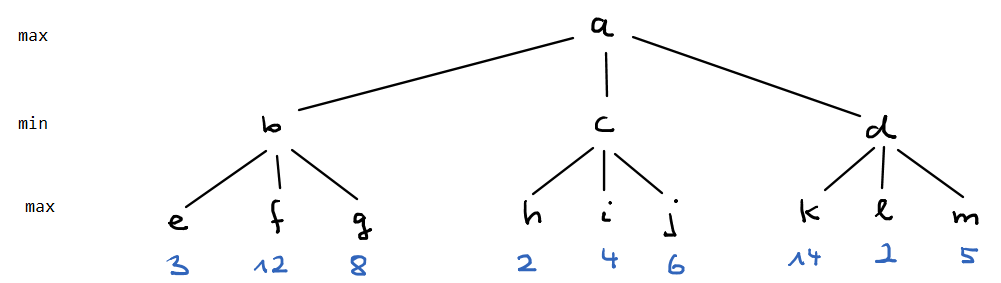
\includegraphics[width=12cm]{bild12.png} 
\end{frame}

\begin{frame}[fragile]
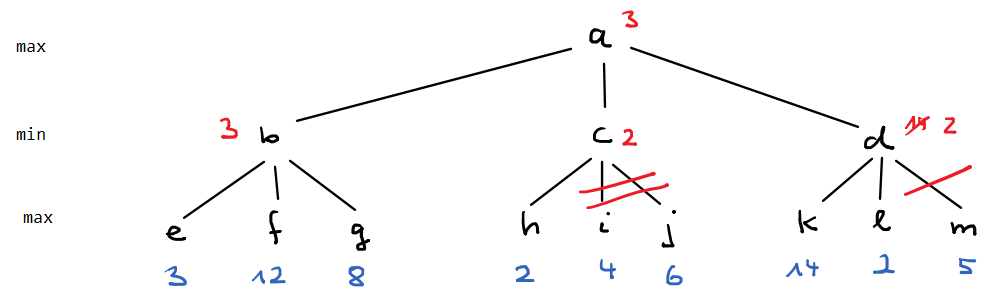
\includegraphics[width=12cm]{bild13.png}  \pause

Dazu wird jedem Knoten ein $\alpha$  und ein $\beta$-Wert mitgegeben, die im Verlauf des Algorithmus upgedated
werden und die es gestatten, ein Kriterium zu formulieren, wann das pruning erfolgen kann.
\end{frame}

%\begin{frame}[fragile]
%Der Alpha-Beta-Algorithmus
%\begin{lstlisting}[basicstyle=\tiny]
%def maximize(state,$\alpha, \beta$):
%    '''
%    state: Spielstellung
%    $\alpha$ die beste bisher Bewertung entlang des Pfads zur Wurzel für den Maximizer. 
%    $\beta$ die beste bisher Bewertung entlang des Pfads zur Wurzel für den Minimizer. 
%    returns: (st, k), die Folgestellung, die die höchste Bewertung k hat
%    '''
%    Falls state ein Blatt, wird keine Folgestellung sondern nur die 
%        Stellungsbewertung zurückgegeben.
%    
%    Von allen Kindern von state wird das mit der höchsten
%        Bewertung des Minimizers gesucht. 
%        Falls sich während dieser Suche herausstellt, das die Bewertung 
%        des Minimizers >= $\beta$, dann wird gepruned
%        Falls sich herausstellt, dass die Bewertung > $\alpha$, dann wird $\alpha$ upgedated
% 
% 
%    
%st =  ...                               # Ausgangsstellung
%besterZug, k = maximize(st,-inf,inf)    # der beste Zug nach st für den Maximizer
%\end{lstlisting} 
%\end{frame}

\begin{frame}[fragile]
Der Alpha-Beta-Algorithmus \\
\begin{minipage}[t]{7.5cm}
\begin{lstlisting}[basicstyle=\tiny]
inf = float('inf')
def maximize(state,alpha,beta):
    if terminal_test(state):
        return None,evaluation(state)
    v, bestChild = -inf, None
    for child in nextstates(state):
        _,utility = minimize(child,alpha,beta)
        if utility > v:
            v, bestChild = utility, child
        if v >= beta:
            break
        if v > alpha:
            alpha = v
    return bestChild, v

def minimize(state,alpha,beta):
    if terminal_test(state):
        return None,evaluation(state)
    v, bestChild = inf, None
    for child in nextstates(state):
        _,utility = maximize(child,alpha,beta)
        if utility < v:
            v, bestChild = utility, child
        if v <= alpha:
            break
        if v < beta:
            beta = v
    return bestChild, v 

# bester folgezug für maximizer nach state
bestnext, _ = maximize(state,-inf,inf)
\end{lstlisting}  
\end{minipage} 
%\begin{minipage}[t]{4cm}
%alpha: die beste bisher untersuchte Option entlang des Pfads zur Wurzel für den Maximizer. 
%~~\\~~\\
%beta: die beste bisher untersuchte Option entlang des Pfads zur Wurzel  für den Minimizer.
%~~\\~~\\
%pruning: \\
%bei max, wenn $v \ge \beta$ \\
%bei min, wenn $v \le \alpha$
%\end{minipage} 
\end{frame}

\begin{frame}[fragile]
Vereinfachte Notation zur Durchführung des Alpha-Beta-Algorithmus:

Zu Beginn ist $\alpha = -\infty$ und $\beta = +\infty$.

$\alpha$ und $\beta$ werden von oben nach unten durchgereicht. Bei den max-Knoten wird $\beta$ nicht verändert, bei den min-Knoten wird $\alpha$ nicht verändert. Wir notieren deshalb nur die $\alpha$-Werte bei den max-Knoten und nur die $\beta$-Werte bei den min-Knoten. An den Blätter notieren wir keine $\alpha$ oder $\beta$-Werte.

Der Algorithmus ist eine Tiefensuche, die abwärts- und aufwärts-Bewegungen macht. Abwärts erben die Kinder ihre  $\alpha$ und $\beta$-Werte von den Großeltern. Wenn aufwärts ein Eltern-Knoten bei einem Kind etwas sieht, was er haben will, nimmt er es von dem Kind.

Wenn an einer Stelle entdeckt wird, dass $\alpha$ größer-gleich dem darüber stehenden $\beta$ ist oder
dass $\beta$ kleiner-gleich dem darüber stehenden  $\alpha$ ist, wird gepruned.

Der Auftraggeber des pruning ist der Vater des Knotens, bei dem das pruning erfolgt.
\end{frame}

\begin{frame}[fragile]
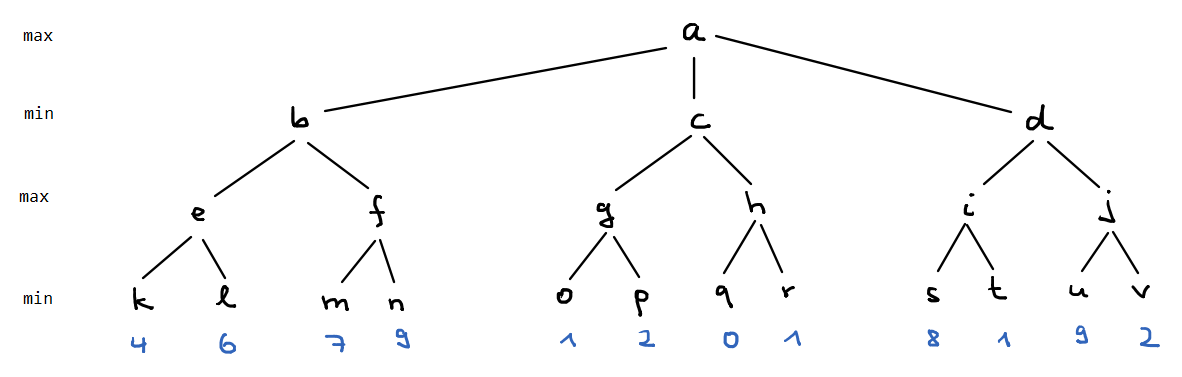
\includegraphics[width=12cm]{bild14.png} 

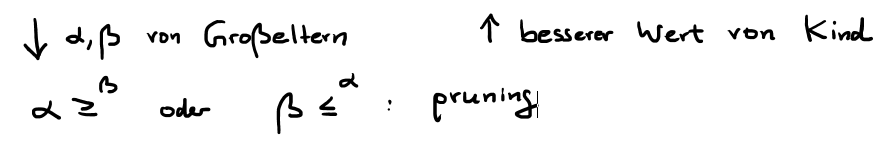
\includegraphics[width=10cm]{kurzform.png} 



\end{frame}

\begin{frame}[fragile]
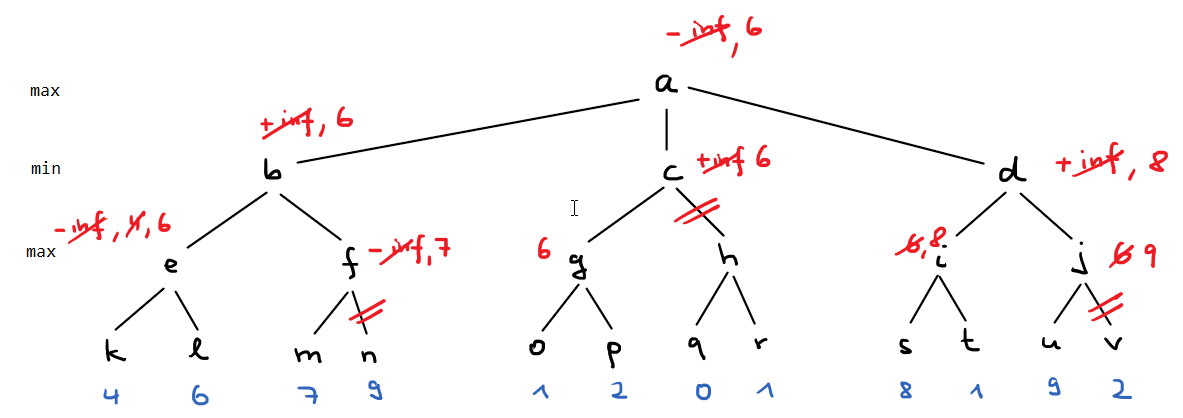
\includegraphics[width=12cm]{bild15a.png} 

Reihenfolge des Blattbesuchs,  \# für pruning:
\begin{lstlisting}
k l m # o p # s t u # 
bester Zug d
\end{lstlisting} 
\end{frame}



 \end{document}